\chapter{Introduction}
\label{ch:introduction}
Robots are becoming a familiar presence in the daily life of people helping
them in different scenarios: warehouses, healthcare, search and rescue and
office robots. \newline
The industrial area is possibly one in which automated machines have had the
most successful applications. Indeed, the 4.0 industrial revolution meant for
many workers an increased level of interaction with the machines present in the
factory \cite{industry4_0}, with a significant impact on
productivity~\cite{coordinationInWarehouse}. One of the most known examples of
robotics applied to the industry is Spot from Boston Dynamics, which not only
can freely move in the environment and record it with its cameras, but can also
find possible problems and predict which components will need maintenance when
integrated with sensors~\cite{bostonDynamics}. This is just an example of how
robotics can be applied to the industrial domain. Indeed, robotics proves to
enhance and solve more and more easily logistics manufacturing problems
allowing for a better use of the industrial
space~\cite{industry4_0_1}.\newline
Since the last decade, robots have been used with great profit in the
healthcare sector. For example, they have been successfully used in precise
surgical procedures to help surgeons reach difficult anatomical compartments
and doing operations that would otherwise be impossible \cite{surgicalRobot}.
Also, robotics has been applied to help elderly and impaired people move more
freely, besides being used to assist during rehabilitation~\cite{friWalker}.
\newline
Another important scenario in which robots have be successfully utilized is
search and rescue missions in challenging environments
\cite{searchRescueDrones}, where the environmental conditions may otherwise
endanger also the rescuers. \newline
Finally, robots can be used to help in the day-to-day life of an office
allowing affairs to sped up and simplifying the general workday~\cite{cobots}.
\newline
In the majority of these situations, there are multiple robots that to complete
one or multiple tasks in the most efficient way possible need to cooperate with 
each other. Moreover, having the robots follow human-aware trajectories, 
dramatically increases the reliability and safety of the environment, while yet
keeping the benefits of using robotics in the scenario. \newline
The focus of this thesis will be the industrial scenario focusing in 
particular on motion planning. The main contribution we have worked on are:
\begin{itemize}
  \item A comprehensive overview of the state of the art regarding techniques 
    and algorithms used to solve motion planning problems, 
    Chapter~\ref{ch:motionPlanning}.
  \item A comparison of some of said techniques addressing a real warehouse
    scenario with the due modifications, Chapter~\ref{ch:solutions}. 
  \item A discussion of the results obtained and the possible problems that
    should be addressed, Chapter~\ref{ch:discussion}.  
\end{itemize}
\begin{figure}[tb]
  \centering
  \includegraphics[width=0.32\textwidth]{warehouse}
  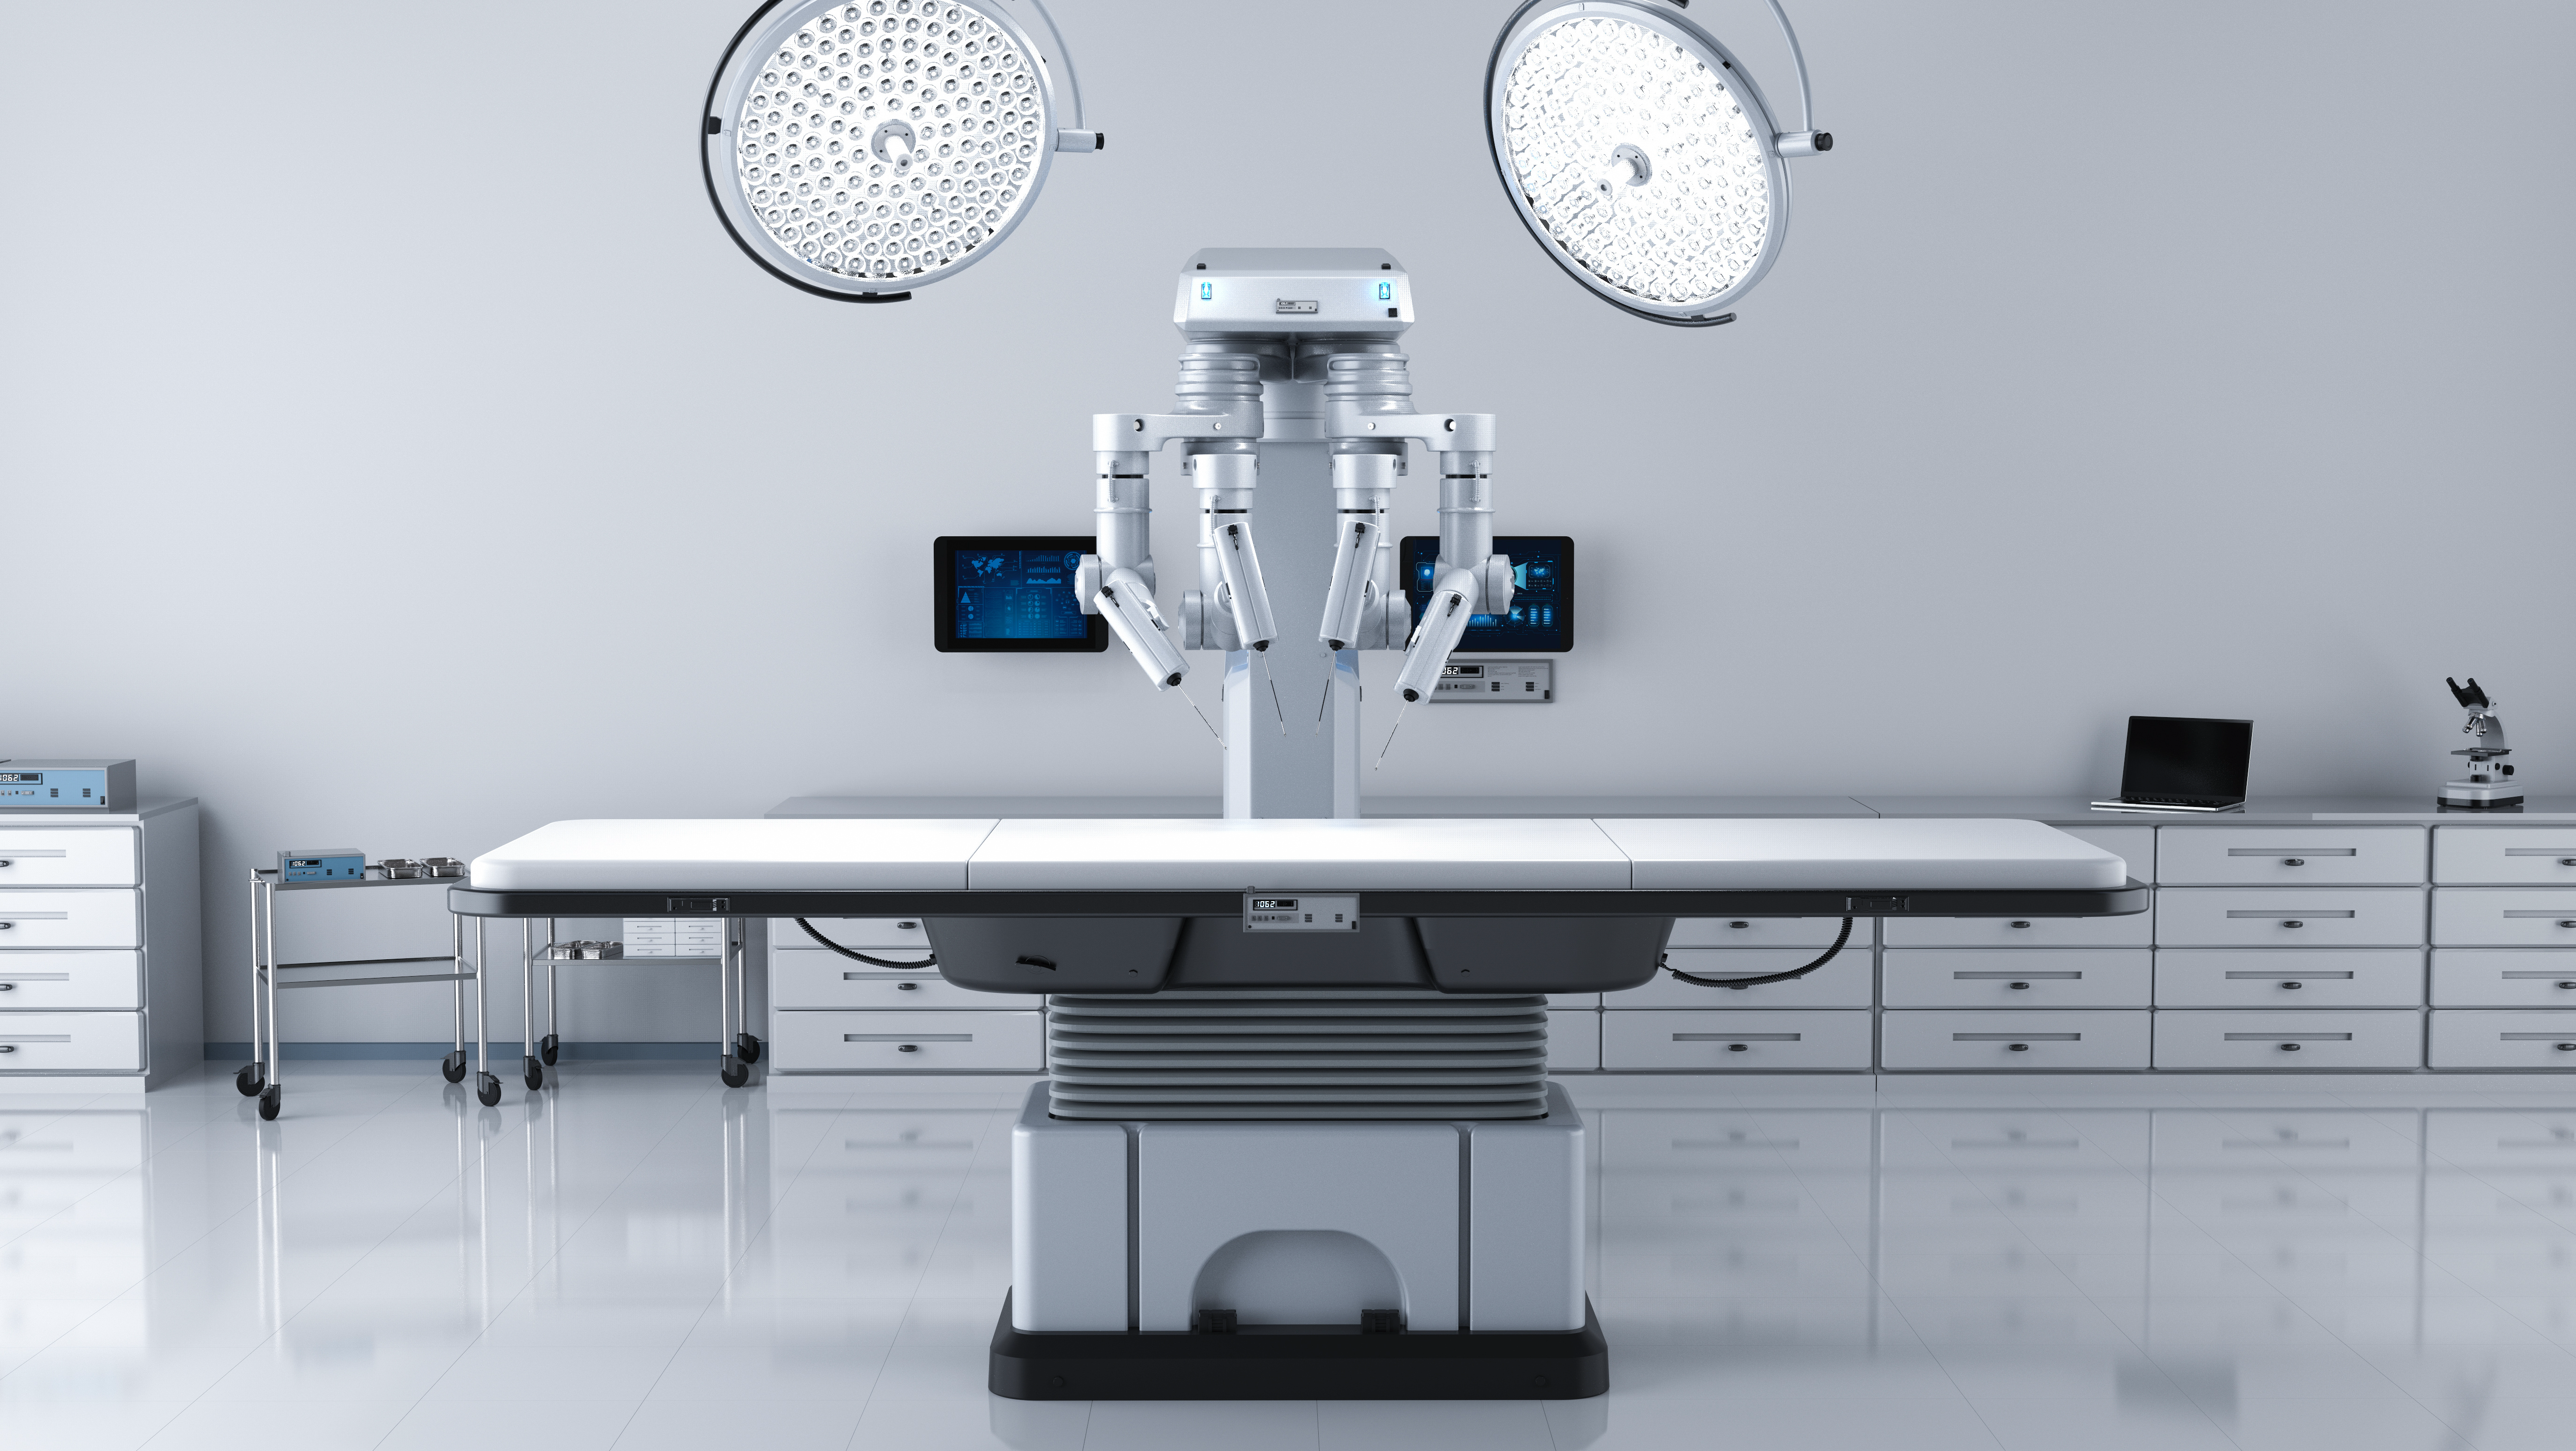
\includegraphics[width=0.32\textwidth]{surgeon1}
  \includegraphics[width=0.32\textwidth]{rescue}
  \caption{Robots can be employed in a different number of scenarios to help
  humans, from the movement of heavy packages in warehouses, to the precision
  of surgery, and also to help search and rescue in remote environments.}
  \label{fig:robot_examples}
\end{figure}
